\section{Algorithm \& Implementation}
\label{sec:algorithm_implementation}


\subsection{Equation Solving}
\label{subsec:equation_solving}
For the following algorithms we need to solve equations involving distance functions \(\delta\). More specifically, we want to solve the following equation 
\begin{equation}
  \delta(u + t \cdot (v - u), w) = \varepsilon \label{eq:eq_solve_main}
\end{equation}
for arbitrary, fixed vectors \(u, v, w \in \R^d\) and fixed \(\varepsilon \in \R_{>0}\) for the variable \(t \in \R\) or determine that there is no such solution. This will have a smallest solution \(\hat{t}_0\) and largest solution \(\hat{t}_1\) in which we are interested. Those two solutions may be the same or may not exist at all.

\begin{figure}
    \centering
    % First row of subfigures
    \begin{subfigure}[b]{0.3\textwidth}
        \centering
        \begin{tikzpicture}
            % Define points
            \coordinate (u)  at (2,0.5);
            \coordinate (u0) at (0,0);
            \coordinate (v) at (4,1);
            \coordinate (w) at (2,0);

            % Draw the line segment from u to v
            \draw[thick] (u) -- (v);

            \draw[thick] (w) circle (1);

            % Find intersection points between the line and the circle
            \path[name path=line] (u0) -- (v);
            \path[name path=circle] (w) circle (1);
            \path[name intersections={of=line and circle, by={t1,t0}}];

            % Label intersection points
            \node[circle,fill,color=red,inner sep=1pt,label={[text=red, below]:\(u=\hat t_0'\)}] at (u) [] {}; 
            \node[circle,fill,color=blue,inner sep=1pt,label={[text=blue]-90:\(v\)}] at (v) [] {}; 
            \node[circle,fill,color=blue,inner sep=1pt,label={[text=blue]-90:\(w\)}] at (w) [] {}; 

            \node[circle,fill,color=red,inner sep=1pt,label={[text=red, above left]:\(\hat t_0\)}] at (t0) [] {}; 
            \node[circle,fill,color=red,inner sep=1pt,label={[text=red, above]:\(\hat t_1=\hat t_1'\)}] at (t1) [] {}; 

            % Draw dotted extensions of the line segment
            \draw[dotted] (u0) -- (u);
            %\draw[dotted] (v) -- ($(v)!-1.5!(u)$);
        \end{tikzpicture}
      \caption{\(\hat t_0 < 0 < \hat t_1 < 1\) \\ \(\hat t_0' = 0, \hat t_1' = \hat t_1\)}
        \label{fig:sub2}
    \end{subfigure}
    \hfill
    \begin{subfigure}[b]{0.3\textwidth}
        \centering
        \begin{tikzpicture}
            % Define points
            \coordinate (u) at (0,0);
            \coordinate (v) at (4,1);
            \coordinate (w) at (2,0);

            % Draw the line segment from u to v
            \draw[thick] (u) -- (v);

            \draw[thick] (w) circle (1);

            % Find intersection points between the line and the circle
            \path[name path=line] (u) -- (v);
            \path[name path=circle] (w) circle (1);
            \path[name intersections={of=line and circle, by={t1,t0}}];

            % Label intersection points
            \node[circle,fill,color=blue,inner sep=1pt,label={[text=blue]-90:\(u\)}] at (u) [] {}; 
            \node[circle,fill,color=blue,inner sep=1pt,label={[text=blue]-90:\(v\)}] at (v) [] {}; 
            \node[circle,fill,color=blue,inner sep=1pt,label={[text=blue]-90:\(w\)}] at (w) [] {}; 

            \node[circle,fill,color=red,inner sep=1pt,label={[text=red, above left]:\(\hat t_0=\hat t_0'\)}] at (t0) [] {}; 
            \node[circle,fill,color=red,inner sep=1pt,label={[text=red, above]:\(\hat t_1=\hat t_1'\)}] at (t1) [] {}; 

            % Draw dotted extensions of the line segment
            %\draw[dotted] ($(u)!-1.5!(v)$) -- (u);
            %\draw[dotted] (v) -- ($(v)!-1.5!(u)$);
        \end{tikzpicture}
        \caption{\(0 < \hat t_0 < \hat t_1 < 1\)\\ \(\hat t_0' = \hat t_0, \hat t_1' = \hat t_1\)}
        \label{fig:sub1}
    \end{subfigure}
    \hfill
    \begin{subfigure}[b]{0.3\textwidth}
        \centering
        \begin{tikzpicture}
            % Define points
            \coordinate (v)  at (2,0.5);
            \coordinate (u) at (0,0);
            \coordinate (v0) at (4,1);
            \coordinate (w) at (2,0);

            % Draw the line segment from u to v
            \draw[thick] (u) -- (v);

            \draw[thick] (w) circle (1);

            % Find intersection points between the line and the circle
            \path[name path=line] (u) -- (v0);
            \path[name path=circle] (w) circle (1);
            \path[name intersections={of=line and circle, by={t1,t0}}];

            % Label intersection points
            \node[circle,fill,color=blue,inner sep=1pt,label={[text=blue, below]:\(u\)}] at (u) [] {}; 
            \node[circle,fill,color=red,inner sep=1pt,label={[text=red, below]:\(v=\hat t_1'\)}] at (v) [] {}; 
            \node[circle,fill,color=blue,inner sep=1pt,label={[text=blue]-90:\(w\)}] at (w) [] {}; 

            \node[circle,fill,color=red,inner sep=1pt,label={[text=red, above left]:\(\hat t_0=\hat t_0'\)}] at (t0) [] {}; 
            \node[circle,fill,color=red,inner sep=1pt,label={[text=red, above]:\(\hat t_1\)}] at (t1) [] {}; 

            % Draw dotted extensions of the line segment
            \draw[dotted] (v) -- (v0);
            %\draw[dotted] (v) -- ($(v)!-1.5!(u)$);
        \end{tikzpicture}
      \caption{\(0 < \hat t_0 < 1 < \hat t_1 \) \\ \(\hat t_0' = \hat t_0, \hat t_1' = 1\)}
        \label{fig:sub3}
    \end{subfigure}

    % Second row of subfigures
    \begin{subfigure}[b]{0.3\textwidth}
        \centering
        \begin{tikzpicture}
            % Define points
            \coordinate (u) at (0,0);
            \coordinate (v0) at (4,1);
            \coordinate (v) at (2,0.5);
            \coordinate (w) at (3,0);

            % Draw the line segment from u to v
            \draw[thick] (u) -- (v);

            \draw[thick] (w) circle (1);

            % Find intersection points between the line and the circle
            \path[name path=line] (u) -- (v0);
            \path[name path=circle] (w) circle (1);
            \path[name intersections={of=line and circle, by={t1,t0}}];

            % Label intersection points
            \node[circle,fill,color=blue,inner sep=1pt,label={[text=blue]-90:\(u\)}] at (u) [] {}; 
            \node[circle,fill,color=blue,inner sep=1pt,label={[text=blue, above]:\(v\)}] at (v) [] {}; 
            \node[circle,fill,color=blue,inner sep=1pt,label={[text=blue]-90:\(w\)}] at (w) [] {}; 

            \node[circle,fill,color=red,inner sep=1pt,label={[text=red, below right]:\(\hat t_0\)}] at (t0) [] {}; 
            \node[circle,fill,color=red,inner sep=1pt,label={[text=red, above]:\(\hat t_1\)}] at (t1) [] {}; 

            % Draw dotted extensions of the line segment
            \draw[dotted] (v) -- (v0);
            %\draw[dotted] (v) -- ($(v)!-1.5!(u)$);
        \end{tikzpicture}
        \caption{\(\hat t_0 < \hat t_1 < 0\)\\ \(\hat t_0' = \hat t_1' = \infty\)}
        \label{fig:sub4}
    \end{subfigure}
    \hfill
    \begin{subfigure}[b]{0.3\textwidth}
        \centering
        \begin{tikzpicture}
            % Define points
            \coordinate (u0) at (-1.5,-0.5);
            \coordinate (u) at (-0.75,-0.125);
            \coordinate (v) at (0.5,0.5);
            \coordinate (v0) at (1.5,1);
            \coordinate (w) at (0,0);

            % Draw the line segment from u to v
            \draw[thick] (u) -- (v);

            \draw[thick] (w) circle (1);

            % Find intersection points between the line and the circle
            \path[name path=line] (u0) -- (v0);
            \path[name path=circle] (w) circle (1);
            \path[name intersections={of=line and circle, by={t1,t0}}];

            % Label intersection points
            \node[circle,fill,color=red,inner sep=1pt,label={[text=red, below right]:\(u=\hat t_0'\)}] at (u) [] {}; 
            \node[circle,fill,color=red,inner sep=1pt,label={[text=red, left]:\(v=\hat t_1'\)}] at (v) [] {}; 
            \node[circle,fill,color=blue,inner sep=1pt,label={[text=blue,right]:\(w\)}] at (w) [] {}; 

            \node[circle,fill,color=red,inner sep=1pt,label={[text=red, left]:\(\hat t_0\)}] at (t0) [] {}; 
            \node[circle,fill,color=red,inner sep=1pt,label={[text=red, right]:\(\hat t_1\)}] at (t1) [] {}; 

            % Draw dotted extensions of the line segment
            \draw[dotted] (u0) -- (v0);
        \end{tikzpicture}
        \caption{\(\hat t_0 < 0 < 1 < \hat t_1\)\\ \(\hat t_0' = 0, \hat t_1' = 1\)}
        \label{fig:sub5}
    \end{subfigure}
    \hfill
    \begin{subfigure}[b]{0.3\textwidth}
        \centering
        \begin{tikzpicture}
            % Define points
            \coordinate (u0) at (-2,-1);
            \coordinate (u) at (1,0.5);
            \coordinate (v) at (2,1);
            \coordinate (w) at (-0.5,0);

            % Draw the line segment from u to v
            \draw[thick] (u) -- (v);

            \draw[thick] (w) circle (1);

            \path[name path=line] (u0) -- (v);
            \path[name path=circle] (w) circle (1);
            \path[name intersections={of=line and circle, by={t1,t0}}];

            \node[circle,fill,color=blue,inner sep=1pt,label={[text=blue]-90:\(u\)}] at (u) [] {}; 
            \node[circle,fill,color=blue,inner sep=1pt,label={[text=blue, above]:\(v\)}] at (v) [] {}; 
            \node[circle,fill,color=blue,inner sep=1pt,label={[text=blue]-90:\(w\)}] at (w) [] {}; 

            \node[circle,fill,color=red,inner sep=1pt,label={[text=red, below left]:\(\hat t_0\)}] at (t0) [] {}; 
            \node[circle,fill,color=red,inner sep=1pt,label={[text=red, left]:\(\hat t_1\)}] at (t1) [] {}; 

            \draw[dotted] (u) -- (u0);
        \end{tikzpicture}
        \caption{\(1 < \hat t_0 < \hat t_1\)\\ \(\hat t_0' =  \hat t_1' = \infty\)}
        \label{fig:sub6}
    \end{subfigure}

    % Third row of subfigures (centered)
    \begin{subfigure}[b]{0.3\textwidth}
        \centering
        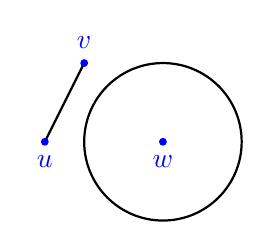
\begin{tikzpicture}
            % Define points
            \coordinate (u) at (1.5,0);
            \coordinate (v) at (2,1);
            \coordinate (w) at (3,0);

            % Draw the line segment from u to v
            \draw[thick] (u) -- (v);

            \draw[thick] (w) circle (1);

            % Label intersection points
            \node[circle,fill,color=blue,inner sep=1pt,label={[text=blue]-90:\(u\)}] at (u) [] {}; 
            \node[circle,fill,color=blue,inner sep=1pt,label={[text=blue, above]:\(v\)}] at (v) [] {}; 
            \node[circle,fill,color=blue,inner sep=1pt,label={[text=blue]-90:\(w\)}] at (w) [] {}; 
        \end{tikzpicture}
        \caption{\(\hat t_0, \hat t_1\) do not exist\\ \(\hat t_0' = \hat t_1' = \infty\)}
        \label{fig:sub7}
    \end{subfigure}
    \caption{The different kinds of solutions. Note that we associate \(0\) with \(u\), \(1\) with \(v\) and \(t\) with \((1-t)u + tv\)}
    \label{fig:main}
\end{figure}

For our use cases we do not need the actual solutions \(\hat{t}_0\) and \(\hat{t}_1\) but modified solutions \(\hat{t}_0'\) and \(\hat{t}_1'\) which are defined as 
\begin{equation}
  \hat{t}_0' \coloneq \begin{cases}
    0 & \textrm{ if } \hat{t}_0 < 0 \textrm{ and } \hat{t}_1 \geq 0\\
    \hat{t}_0 & \textrm{ if } \hat{t}_0 \in [0, 1]\\
    \infty &\textrm{ otherwise }
  \end{cases}\\
  \hat{t}_1' \coloneq \begin{cases}
    1 & \textrm{ if } \hat{t}_1 > 1 \textrm{ and } \hat{t}_0 \leq 1\\
    \hat{t}_1 & \textrm{ if } \hat{t}_1 \in [0, 1]\\
    \infty &\textrm{ otherwise }
  \end{cases},
\end{equation}
where the \emph{otherwise} case also includes the case of there being no solution to \cref{eq:eq_solve_main}. 
For a line segment \(\overline{uv}\) and a point \(w\) we denote \(\hat t_0'(\overline{uv}, w)\) and \(\hat t_1'(\overline{uv}, w)\) to be the respective modified solutions for the given line segment and point. We do not include \(\varepsilon\) in that notation as it is fixed throughout all algorithms and thus needs to disambiguation.

In general, determining these solutions requires finding roots of polynomials and thus there is no exact solution algorithm for distances derived from the norms \(L_e\) for \(e > 4\) as such polynomials are not solvable. Here, we derive explicit solutions for the Euclidean Distance, the Manhattan Distance and the Chebyshev Distance. 


This gives us the following six cases 
\begin{enumerate}
  \item \(\hat t_1 < 0\) in which case we want to report that there is no solution.
  \item \(0 = \hat t_0 < \hat t_1 < 1\) in which the solution pair is \((0, \hat t_1)\).
  \item \(0 = \hat t_0 < \hat t_1 = 1\) in which the solution pair is \((0, 1)\).
  \item \(0 < \hat t_0 < \hat t_1 < 1\) in which the solution pair is \((\hat t_0, \hat t_1)\).
  \item \(0 < \hat t_0 < \hat t_1 = 1\) in which the solution pair is \((\hat t_0, 1)\).
  \item \(\hat t_0 > 0\) in which case we want to report that there is no solution.
\end{enumerate}

Case \(3\) is trivial for all distances and does not require solving an equation. Cases \(2, 4\) and \(5\) happen if there are solutions in the interval and optionally one of the distances \(\delta(u,w) < \varepsilon\) or \(\delta(v,w) < \varepsilon\).


\subsubsection{Euclidean Distance}
\label{subsubsec:eq_euclidean_distance}
In the case of the Euclidean distance, \cref{eq:eq_solve_main} simplifies to the equation 
\begin{align*}
  \| (u - w) + t(v - u) \|_2 &= \varepsilon \\
  \| (u - w) + t(v - u) \|_2^2 &= \varepsilon^2 \\
  \| u - w \|_2^2 + 2\braket{u - w | v - u} t  +  \| v - u \|_2^2 t^2 &= \varepsilon^2 \\
  \underbrace{\delta(u,w)^2 - \varepsilon^2}_{\alpha_0} + \underbrace{2\braket{u - w | v - u} }_{\alpha_1}t  +  \underbrace{\delta(v, u)^2}_{\alpha_2} t^2 &= 0 \\
  \alpha_0 + \alpha_1 t  + \alpha_2 t^2 &= 0,
\end{align*}

which is a quadratic equation in \(t\) and can be solved explicitly as 

\begin{equation}
  t_{0,1} = \frac{-\alpha_1 \pm \sqrt{\alpha_1^2 - 4\alpha_0\alpha_2}}{2\alpha_2}.\label{eq:sol_explicit_euclidean}
\end{equation}

If the discriminant \(\alpha_1^2 - 4\alpha_0\alpha_2\) is smaller than \(0\) there is no solution. Otherwise we can compute the two solutions and have the lower and smallest and largest solution. These values might need to be clamped to be between \(0\) and \(1\). 


\subsubsection{Manhattan Distance}
\label{subsubsec:eq_manhattan_distance}
In the case of the Manhattan distance, \cref{eq:eq_solve_main} simplifies to 
\begin{equation}
  \sum_{i=0}^d |u_i - w_i + t (v_i - u_i)| = \varepsilon. \label{eq:solve_manhattan}
\end{equation}

We note that \(|u_i - w_i + t (v_i - u_i )|\) can only assume the two values \(u_i - w_i + t(v_i - u_i)\) or \(w_i - u_i - t(v_i - u_i)\) depending on \(t\). For a fixed \(t\) we can evaluate all terms in the sum in \cref{eq:solve_manhattan} to get a linear equation in \(t\) which is trivial to solve, and the check if the resulting solution is valid. We define \(t_i \coloneq \frac{w_i - u_i}{v_i - u_i} \). Let \(\sigma:\set{1,\dots, d} \to \set{1,\dots, d}\) be the sorting permutation with \(t_{\sigma(1)} < t_{\sigma(2)} < \cdots < t_{\sigma(d)}\). For \(t \in [t_{\sigma(i)}, t_{\sigma(i+1)}]\) each of the terms in the sum can be simplified to a linear term without the absolute value and thus the whole sum degenerates into a linear equation which can be trivially solved. Finally we can check if the solution found for this interval does indeed lie in the interval. 

This whole process can be implemented na\"ively using a Sweepline algorithm in time \(\O(d^2)\) by constructing the values \(t_i\), sorting them and for each interval we compute the whole sum in linear time and solve the equation. As there are \(d\) many such values to consider we get quadratic runtime. We can improve this by using the fact that by iterating from smallest to largest during each testing step only a single term changes its sign, thus we can maintain the current linear equation and update it accordingly in constant time. The bulk of the computation now lies in sorting which gives us a runtime og \(\O(d \log d)\). 

Let us consider the non-trivial cases we defined earlier. Case \(4\) is the only case where we find two solutions in the interval and is thus covered. In cases \(2\) and \(5\) only one solution will be found and one of the distances will be smaller \(\varepsilon\). In the other two cases no solution will be found so the behaviour of returning no answer is correct.

There are a few edge cases, namely those being that multiple \(t_i\) coincide as well as that there are \(u_i = v_i\). The former case can easily be handled by treating all terms with the same value for \(t_i\) as a single term. The second case degenerates the term into a constant which can be pulled out of the sum and into the right side.

\begin{algorithm}[ht]
  \DontPrintSemicolon
  \KwData{vectors \(u, v, w \in \R^d\), \(\varepsilon > 0\)}
  \KwResult{Solution to \cref{eq:solve_manhattan}}
  \BlankLine
  \(global\_slope \gets 0, global\_offset \gets 0\) \;
  \(events \gets Array(d)\)
  \For{\(i = 1, \dots, d\)}{
    \(slope \gets v_i - u_i, offset \gets u_i - w_i\)\;
    \If{\(slope < 0\)}{
      \(slope \gets -slope, offset \gets -offset\)
    } \ElseIf{\(slope = 0\)}{
      \(\varepsilon \gets \varepsilon - |offset|\)\;
      \Continue
    }
    \(zero \gets - \frac{offset}{slope}\)\;
    \If{\(zero \leq 0\)}{
      \(global\_offset \gets global\_offset + offset\)\;
      \(global\_slope \gets global\_slope + slope\)\;
      \Continue
    } 
    \(global\_offset \gets global\_offset - offset\)\;
    \(global\_slope \gets global\_slope - slope\)\;
    \If{\(zero \geq 1\)}{
      \Continue
    }
    \(events.append((zero, slope, offset))\)\;
  }
  Sort \(events\) by their \(zero\) component\;
  \(start \gets 0\)\;
  \For{\((zero, slope, offset) \in events\)}{
    Test if solution \(\frac{\varepsilon - global\_offset}{global\_slope} \in [start, zero]\) and report solution if so\;
    \(global\_offset \gets global\_offset + 2offset\)\;
    \(global\_slope \gets global\_slope + 2slope\)\;
    \(start \gets zero\)
  }
  Test if solution \(\frac{\varepsilon - global\_offset}{global\_slope} \in [start, 1]\) and report solution if so\;

  \caption{manhattan\_solver(\(u, v, w, \varepsilon\))}
  \label{algo:solve_manhattan}
\end{algorithm}


\subsubsection{Chebyshev Distance}
\label{subsubsec:eq_chebyshev_distance}
In the case of the Chebyshev distance \cref{eq:eq_solve_main} becomes 
\begin{equation}
  \max_{i = 1,\dots, d} |u_i - w_i + t(v_i - u_i)| = \varepsilon\label{eq:solve_chebyshev}
\end{equation}
which a na\"ive solution can be found easily as the maximum will only assume as value one of the terms and each term has two possible values depending on the absolute value. Thus there are \(2d\) possible solutions which can be checked each in linear time if they indeed are the maximum resulting in a simple quadratic runtime algorithm. 

Just as in the case of the Manhattan distance, we only need to consider the solutions in the interval \([0,1]\) which eliminates possible solutions and in small dimensions this is probably the best choice. 

We can also reduce the runtime to \(d \log d\) by efficiently updating the current maximum. As each term is a line, we can find the initial maximum line at the start and update it when it crosses another line thus a modified version of the Bentley-Ottmann algorithm for line segment intersection can be used where where the handling of intersections is modified to remove the line segment that falls below the other and only computing new intersections upwards. This guarantees that even if there are quadratically many intersecions only \(\O(d \log d)\) runtime is needed as irrelevant intersections are omitted. 
This allows a simplification in that we do not need a self-balancing binary search tree to store the line segments. A doubly linked list suffices as we remove for each intersection a line segment and the relative ordering remains the same. This list can be stored in an array where each array entry has an index to the previous and next line segment and its data, i.e., the offset and slope. A more detailed version of this idea can be seen in \cref{algo:solve_chebyshev}. For a full implementation, the case distinction in \cref{subsec:equation_solving} needs to be implemented, the handling of the marked solutions.

\begin{algorithm}[ht]
  \DontPrintSemicolon
  \KwData{vectors \(u, v, w \in \R^d\), \(\varepsilon > 0\)}
  \BlankLine
  \(candidates \gets \set{(2i, u_i - w_i, v_i - u_i), (2i+1, w_i - u_i, u_i - v_i) | i = 0, \dots, d - 1}\) \;
  \(queue \gets PriorityQueue()\) \;
  \(list \gets Array(|candidates|)\) \;
  sort candidates according to second component descendingly,
  in case of ties use the third component as tie breaker descendingly \;
  \(PREV \gets 0, NEXT \gets 1\) \tcp{constants for readability}
  \(curr \gets -1\) \;
  \For{\((i, a, b) \in candidates\)}{
    \If{\(curr = -1\)} {
      \(curr \gets i, a' \gets a, b' \gets b\)\;
      \(list[curr] \gets (-1, -1, a, b)\) \;
      \Continue
    } 

    \If{\( a' + b' \geq a + b\)}{
      \Continue \tcp{new line fully below current line so never maximum}
    } 

    \(list[curr][NEXT] \gets i, list[i] \gets (curr, -1, a, b)\) \;
    \(intersection \gets \frac{a' - a}{b - b'}\) \tcp{always in \([0,1]\)}
    \(queue.insert\_with\_priority((curr, i), intersection)\) \;
    \(curr \gets i, a' \gets a, b' \gets b\) \;
  }

  \caption{chebyshev\_solver\_initialization(\(u, v, w\))}
  \label{algo:solve_chebyshev_init}
\end{algorithm}

\begin{algorithm}[ht]
  \DontPrintSemicolon
  \KwData{vectors \(u, v, w \in \R^d\), \(\varepsilon > 0\)}
  \KwResult{Solution to \cref{eq:solve_chebyshev}}
  \BlankLine
  \(chebyshev\_solver\_initialization(u, v, w)\) \;
  \(last\_intersection \gets 0\) \;
  \While{\(\lnot queue.empty()\)}{
    \((i, j), intersection \gets queue.poll()\) \;
    \If{\(list[i][PREV] = -1 \lor list[j][PREV] = -1\)}{
      \Continue \tcp{One of the lines already removed, no intersection}
    } 
    \If{\(i = HEAD\)}{
      \(HEAD \gets j\) \;
      \(\_, \_, a, b \gets list[i]\) \;
      \If{\(b = 0\)}{
        \If{\(a = \varepsilon\) }{
          Mark \(last\_intersection\) as earliest solution or \(intersection\) as last solution \;
        }
        \(last\_intersection \gets intersection\) \;
        \Continue 
      }
      \(solution \gets \frac{\varepsilon - a}{b}\) \;
      Mark \(solution\) as earliest or last solution if \(solution \in [last\_intersection, intersection]\) \;
      \(last\_intersection \gets intersection\) \;
      \Continue
    }
    \(before_i \gets list[i][PREV]\) \;
    \(list[before_i][NEXT] \gets j, list[j][PREV] \gets before_i\) \;
    \(list[i][PREV] \gets -1\) \tcp{mark as removed}
    \(last\_intersection \gets intersection\) \;
    \If{\(before_i \neq HEAD\)}{
      \(\_, \_, a, b \gets list[j]\) \;
      \(\_, \_, a', b' \gets list[before_i]\) \;
      \(intersection \gets \frac{a' - a}{b - b'}\) \tcp{also in \([0,1]\)}
      \(queue.insert\_with\_priority((before_i, j), intersection)\) \;
    }
  }
  Check for solution in \([last\_intersection, 1]\) \;

  \caption{chebyshev\_solver(\(u, v, w, \varepsilon\))}
  \label{algo:solve_chebyshev}
  
\end{algorithm}

\subsection{\(\O(k^*n^5)\) Algorithm}
\label{subsec:simple_algo}

In this subsection we will sketch \citeauthor{on_optimal_polyline_simplification_using_the_hausdorff_and_frechet_distance}'s algorithm for polyline simplification as well as a simplified version of \citeauthor{computing_the_frechet_distance_between_two_polygonal_curves}'s algorithm to decide if two polylines have Fréchet distance of at most \(\varepsilon\). 

\subsubsection{Fréchet Distance Decision Algorithm}
\label{ssec:alt_godau}
The simplification algorithm we will describe heavily uses a subroutine to solve the following problem: Given \(\varepsilon > 0\), a polyline \(P \) of length \(p\), a polyline segment \(P[j' + t' \dots j+1]\) and a line segment \(\overline{P(i')P(i)}\) for \(i' < i \leq p, j' \leq j < p\in \N\) and \(t \in [0, 1]\). Decide if there is a \(t' \in [0, 1]\) such that \(\delta^F(P[j' + t' \dots j + t], \overline{P(i')P(i)}) \leq \varepsilon\) and if so determine the smallest such \(t\).  

This can be solved by a simplified version of \citeauthor{computing_the_frechet_distance_between_two_polygonal_curves}'s algorithm to decide if the Fréchet distance of two polylines is at most \(\varepsilon\). We present the algorithm in the specific form needed for this problem. 

In both cases we require that \(\delta(P(j' + t'), P(i')) \leq \varepsilon\) as the starting points of both polylines must match by definition. If this is not the case we can return that there is no such \(t\). We set \(t_0 \coloneq \hat t_0'(\overline{P(j)P(j+1)}, P(i))\) and \(t_1 \coloneq \hat t_1'(\overline{P(j)P(j+1)}, P(i))\). As the end points must match, we get that \(t \in [t_0, t_1]\). Thus if there are no such interval we can also return that there is no solution.

We distinguish the two cases \(j' = j\) and \(j' < j\). 
\begin{enumerate}
  \item[\(j' = j\): ] In this case both \(t'\) and \(t\) lie on the same line segment \(\overline{P(j)P(j+1)}\) (which is the only line segment of the polyline segment). The only constraints on \(t\) are that \(t \in [t', 1]\) and \(t \in [ t_0, t_1]\) which is possible if and only if \(t' \leq t_1\). If this is the case the solution is \(\max(t', t_0)\).

  \item[\(j' < j\): ] In this case we iterate over all points of the polyline segment \(P(k) = P(j'+1), \dots, P(j)\) and compute the solutions \(\hat t_0(\overline{P(i')P(i)}, P(k)), \hat t_0(\overline{P(i')P(i)}, P(k))\). We maintain the first reachable point \(t'\) (initially \(0\)) on the line segment \(\overline{P(i')P(i)}\) for these points and test if \(t' \leq \hat t_0(\overline{P(i')P(i)}, P(k))\). If that is the case we can update it \(t' \gets \max(t', \hat t_0(\overline{P(i')P(i)}, P(k)))\). If this is not possible at any step we can return that there is no solution. Otherwise, we have fully traversed the line segment and most of the polyline segment. At this point the solution is merely \(t_0\).
\end{enumerate}

\subsubsection{Polyline Simplification Algorithm}
\label{ssec:simple_algo_main}



\subsection{Optimizations}
\label{ssec:optimizations}
Based on the just described algorithm we outline optimizations that greatly reduce the \(\O(k^*n^5)\) runtime in practice or improve upon the algorithm in terms of space and numerical stability. The most effective optimizations circumvent the theoretical runtime by skipping iterations. 

We first note that for the entry \((k, i, j)\) in the dynamic program we do not always need to iterate over all possible \(i' < i\) and \(j' \leq j\). As we are interested in the minimal value \(t\) on the line segment \(\overline{v_{j}v_{j+1}}\) that can be reached, we can stop further search if we have reached a lower bound for that value. Such a lower bound is \(\hat t_0'(\overline{v_{j}v_{j+1}}, i)\), i.e. the modified solution to the \cref{eq:eq_solve_main}, which is tight as for a sufficiently large \(k\) this value must be reached eventually. This allows an early break out of the search through the \(i' < i, j'\leq j\) and a speed up of upto quadratic runtime. 

Another optimization based on a similar insight is the following: If the entry at \((k-1, i, j) = \hat t_0'(\overline{v_{j}v_{j+1}}, i)\), i.e., we have found a simplification for the same \(i\) and \(j\) that has already reached the optimal value, we know this cannot be improved in the current layer \(k\) or any further one. This means, the entry at \((k, i, j)\) can never be used by some entry \((k + 1, i'', j'')\) because of minimality as any such entry that uses \((k, i, j)\) could have already used \((k-1, i, j)\) for \((k, i'', j'')\). This allows us to completely ignore the computation of the value. This allows a continuous speed up of the algorithm while it runs as once this happens for an entry, it will happen for all further ones with a higher value of \(k\) so with each layer more entry computations can be skipped. 

A last simple optimization of a similar type which is particularly useful for well-behaved polylines is to not even start the iterations over the \(i', j'\) if there is no solution \(\hat t_0'(\overline{v_{j}v_{j+1}}, i)\). This happens often if there are not too many line segments close to each other.











%\subsection{Cubic Runtime Algorithm}
%\label{subsec:refined_algo}

\subsection{Implementation}
\label{subsec:implementation}
% details 
% decision problem: is which intersection point comes first instead of explicit computation 
%   does not need sqrt for euclidean distance, no roots for general norms, allows binary search to estimate intervals 
%   only using the distance function instead of root solving algorithm 
%
% only use min(p, q) space instead of p * q space for decision variant (especially for our case constant extra space)
%


